\documentclass{beamer}
\usetheme{Berkeley}

\usepackage{tikz}
\usetikzlibrary{matrix, positioning, fit}

\title{CUMU}
\subtitle{userspace CUDA emulator}
\date{May 13, 2023}

\begin{document}
\begin{frame}
  \titlepage
\end{frame}

\begin{frame}
  \frametitle{why}
  \begin{alertblock}{current situation}
    CUDA is the de-facto API for GPU accelerated application \\
    however proprietary and deeply tied to NVIDIA hardware
  \end{alertblock}
  \begin{block}{alternatives}
    HIP/SYCL/OpenCL/Vulkan Compute \\
    mostly requires code change \\
    with weaker ecosystems
  \end{block}
  \begin{exampleblock}{what if}
    a CUDA implementation that interoperates with existing codes
    a perfect chance to upset Jensen Huang
  \end{exampleblock}
\end{frame}

\begin{frame}
  \frametitle{whom}
  \begin{block}{me}
    experiment NCCL without CUDA capable hardware
  \end{block}
  \begin{block}{linux distributions}
    ease the testing of CUDA based softwares
  \end{block}
  \begin{block}{researchers}
    a deep dive into CUDA internals
  \end{block}
\end{frame}

\begin{frame}
  \frametitle{how}
  \begin{columns}
    \begin{column}{0.3\linewidth}
      \begin{center}
      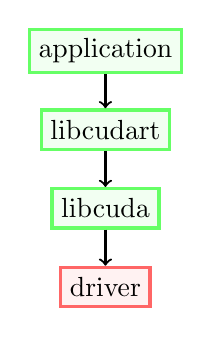
\begin{tikzpicture}[
        node distance=1cm,
        knode/.style={rectangle, draw=red!60, fill=red!5, very thick, minimum size=5mm},
        unode/.style={rectangle, draw=green!60, fill=green!5, very thick, minimum size=5mm},
      ]

        \node[unode] (app)                      {application};
        \node[unode] (cudart) [below of=app]    {libcudart};
        \node[unode] (cuda)   [below of=cudart] {libcuda};
        \node[knode] (kmod)   [below of=cuda]   {driver};

        \draw[thick, ->] (app.south)    -- (cudart.north);
        \draw[thick, ->] (cudart.south) -- (cuda.north);
        \draw[thick, ->] (cuda.south)   -- (kmod.north);
      \end{tikzpicture}
      \end{center}
    \end{column}
    \begin{column}{0.7\linewidth}
      \begin{block}{libcudart}
        CUDA Runtime Library
      \end{block}
      \begin{block}{libcuda}
        CUDA Driver Library
      \end{block}
      The runtime API eases device code management by providing implicit initialization, context management, and module management. \\
      And by reimplementing libcuda, everything atop just works.
    \end{column}
  \end{columns}
\end{frame}
\begin{frame}
  \frametitle{were}
  \begin{block}{CUDA deviceemu}
    the official CUDA emulator at CUDA 3.0
  \end{block}
  \begin{exampleblock}{https://github.com/vosen/ZLUDA}
    a drop-in replacement for CUDA on Intel GPU
  \end{exampleblock}
  \begin{block}{https://github.com/gtcasl/gpuocelot}
    a dynamic compilation framework for PTX
  \end{block}
  \begin{itemize}
    \item varying degrees of success
    \item mostly discontinued
  \end{itemize}
\end{frame}
\begin{frame}
  \frametitle{whoops}
  \begin{alertblock}{Jensen Huang tries his best to stop us}
  \end{alertblock}
  \begin{itemize}
    \item \texttt{dlsym} $\rightarrow$ \texttt{cuGetProcAddress}
    \item \texttt{cuGetExportTable} symbol name $\rightarrow$ uuid
    \item \ldots
  \end{itemize}
\end{frame}
\end{document}
